\documentclass[12pt]{scrreport} 

% Set up styles.
\usepackage[language=english, type=bachelor]{universitystyle} % language may be romanian or english (default is english), type may be bachelor or master (default is bachelor)
% Custom packages.
\usepackage{fancyhdr}
\usepackage{tabularx}
\usepackage{array}
\usepackage{minted}

% Centered table with X column type.
\newcolumntype{Y}{>{\centering\arraybackslash}X}
\usepackage{graphicx}
\graphicspath{ {./pictures/} }

% Latex fixes for sucking.
\usepackage{float}
\usepackage{longtable}
\usepackage[table,xcdraw]{xcolor}
\usepackage{indentfirst}

% Set up the article.
\pagestyle{fancy}
\lhead{}
\chead{}
\renewcommand{\headrulewidth}{0.2pt}
\renewcommand{\footrulewidth}{0.2pt}

\begin{document}

% Title page.
\specialization{ENGLISH}	
\title{Design, implementation and comparision of different software emulating methods}					   
\author{Oniga Andrei-Mihai}											
\supervisor{Lect. dr. Mihai Andrei}				
				
\maketitle

\newpage
\thispagestyle{empty}
\mbox{}
\newpage
\pagenumbering{roman}

% Abstract.
\cleardoublepage
ABSTRACT
\vspace{0.5cm}	
\hrule
\vspace{0.5cm}

\par This thesis explores foundational software emulation techniques, with a particular focus on interpretation and just-in-time (JIT) compilation. The objective is to examine the trade-offs between these approaches in terms of performance and implementation complexity, 

\par To evaluate these techniques in a controlled and educational context, interpreters and JIT compilers were implemented for two minimalistic and well-documented languages, especially well suited to beginners in emulation and thereby offering a comprehensive introduction to emulator design: \textit{Brainfuck and CHIP-8}. They have been selected due to their simplicity, which enables the study to center on emulator behavior rather than language-specific intricacies.

\par The paper's analysis includes performance benchmarking, implementation complexity, and the impact of a selection of optimizations such as instruction folding, jump precalculation, hot loop replacement, and efficient register allocation in the case of JITs. Empirical results also demonstrate that JIT compilation significantly outperforms interpretation, particularly for longer-running programs, primarily due to reduced instruction-fetching and decoding overhead.

\par However, the study also highlights diminishing returns from aggressive optimization strategies such as excessive hot loop replacement which eventually leads to scenarios where entire programs are reduced to singular instructions, limiting further gains. Additionally, some code replacements were found to generate equivalent machine code to the original instruction sequences, rendering the optimization ineffective while increasing code complexity.

\par These findings underscore the balance between simplicity and performance, while aiming to offer accessible insights for readers new to emulation concepts, particularly those engaged in experimental or hobbyist development with languages like the two selected languages.

\par All components discussed have been implemented within a dedicated \textit{C} application, whose architectural design and implementation details are thoroughly documented and analyzed. This practical framework serves to illustrate the theoretical concepts presented, providing a concrete basis for understanding the trade-offs and design decisions inherent in emulator development.

\vspace{0.5em}

\textit{Note: Some of the paper's content has been rewritten and refined to enhance academic clarity and tone by an AI language model. All of the ideas and their implementations have been originally thought of and implemented by the author.}

\vspace{0.5em}

\textbf{Keywords}: software emulation, interpretation, JIT compilation, Brainfuck, CHIP-8, C, performance analysis, optimization techniques

% Table of contents.
\tableofcontents
\newpage
\pagenumbering{arabic}

% Contents.
\chapter{Introduction}
\label{chap:ch1}

\section{About}
\label{chap:ch1sec1}

\par Introducere: obiectivele lucrării și descrierea succintă a capitolelor, prezentarea temei, prezentarea contribuției proprii, respectiv a rezultatelor originale și menționarea (dacă este cazul) a sesiunii de comunicări unde a fost prezentată sau a revistei unde a fost publicată.

\section{Related work}
\label{chap:ch1sec2}

\par CHIP8 Applications in engineering \cite{Chip8Applications2019}.
Brainfuck in reinforcement learning \cite{BFReinforcementLearining2022}.
Esoteric languages list with BF in it \cite{BFEsolang2015}.
Brainfuck conceputal \cite{BFConceptual2017}.
Brainfuck hardware \cite{BFHardware2016}.

\begin{figure}[htbp]
	\centering
		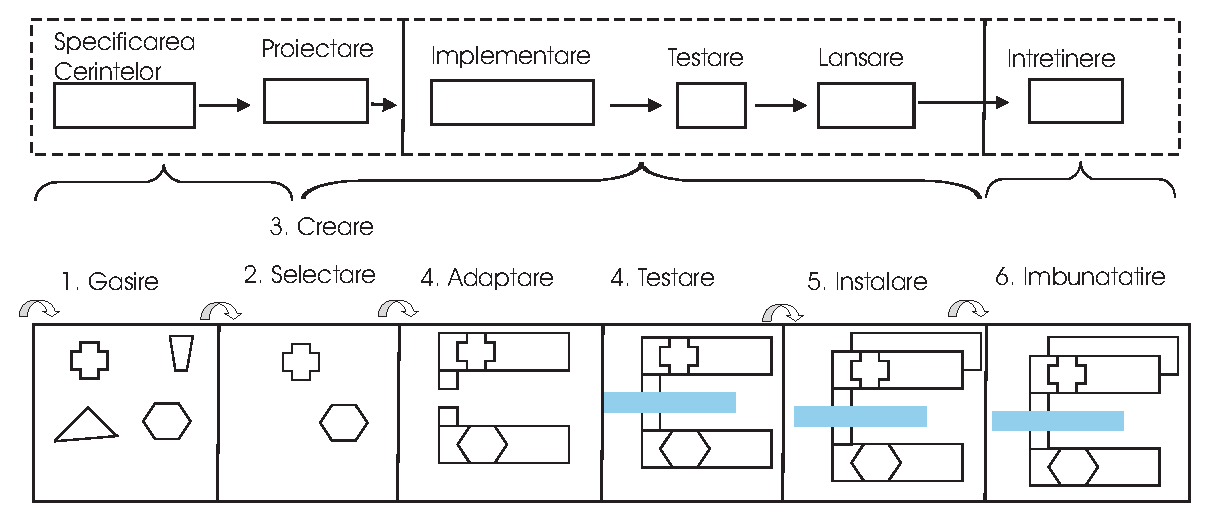
\includegraphics[scale=0.65]{./figures/fig_3_1.eps}
	\caption{Ciclul de dezvoltare al sistemelor bazate pe componente adaptat modelului cascadã}
	\label{FigCBSD}
\end{figure}

Inserarea și Referirea la Tabelul \ref{TabelSolutii}. 

\begin{table}[htbp]
\begin{center}
\begin{tabular}
{|p{120pt}|p{120pt}|p{120pt}|}
\hline
 Nume algoritm  &  Toate soluțiile &  Soluția optimã\\
\hline 
\hline Nume 1 & $20$ & $5$  \\
\hline Nume 2 & $20$ & $2$  \\
\hline
\end{tabular}
\end{center}
\caption{Soluții obținute }
\label{TabelSolutii}
\end{table}


Adaugarea și Referirea la o Ecuație \ref{LabelMyEquation}.


 \begin{equation}
     ws_N4 = w_{14}*N1 + W_{24}+N2 + w_{34}*N3
\label{LabelMyEquation}
 \end{equation}

\clearpage

\chapter{Brainfuck}
\label{chap:ch2}

\par Brainfuck (commonly abbreviated as BF in academic literature) is an esoteric programming language created in 1993 by Swiss computer science student Urban Müller\\\cite{BFWiki}. It was conceived as a minimalist language that challenges conventional programming approaches by reducing syntactic elements to the bare essentials. The language's primary intent is not practical software development, but rather to serve as a vehicle for exploring computational theory, language design, and the boundaries of human-readable code.

\par Brainfuck operates on a simple model of computation: a one-dimensional array of values initialized to zero, and a single data pointer that traverses this memory. Loops in Brainfuck are defined by matching \texttt{[} and \texttt{]} brackets, executing the enclosed code as long as the current cell is non-zero. The language lacks named variables, functions, or high-level abstractions, requiring the programmer to construct all control flow and data manipulation manually.

\par Despite its extreme simplicity, Brainfuck is Turing-complete. This implies that, in theory, any computable function can be implemented using Brainfuck, provided unlimited memory and time. The Turing-completeness of Brainfuck underscores its value as a pedagogical tool, illustrating how a minimal set of operations can express any arbitrarily complex computation.

\par The language's deliberately obfuscated syntax forces programmers to think at the level of memory and instruction cycles, drawing parallels with low-level systems programming, particularly in assembly or machine code. This requirement to engage directly with memory manipulation and flow control makes Brainfuck a unique platform for studying program optimization, instruction translation, and interpreter design.

\par In contemporary settings, Brainfuck is primarily used for educational and experimental purposes. It remains a popular subject in programming contests, obfuscation challenges, and academic discourse within the esoteric programming language (esolang) community. Its design exemplifies the power of minimalism in programming language theory and continues to inspire discussions on language expressiveness, compiler construction, and the boundaries of syntactic design.

\section{Machine specification}
\label{sec:ch2sec1}

\par The language is defined by an extremely compact instruction set consisting of only eight commands:

\begin{table}[H]
\centering
\begin{tabularx}{\textwidth}{| c | Y |}
\hline
+ & Increments the value at the current position that the machine points to. \\ \hline
- & Decrements the value at the current position that the machine points to. \\ \hline
\textless & Moves the pointer one cell to the left.                                  \\ \hline
\textgreater & Moves the pointer one cell to the right.                                 \\ \hline
[ & Jumps after the corresponding closed bracket when the value at the current cell is 0. \\ \hline
] & Jumps after the corresponding open bracket when the value at the current cell is not 0.   \\ \hline
. & Outputs the value at the current cell. \\ \hline
, & Read a value to be placed at the current cell. \\ \hline
\end{tabularx}
\caption{Brainfuck commands and their descriptions.\cite{BFWiki}}
\end{table}

\par The size and number of memory cells in the language are not strictly defined and are typically left to the discretion of the programmer. In the context of this implementation, a memory model consisting of \textit{65,536} cells was adopted (corresponding to the addressable range of a 16-bit pointer) with each cell represented as an unsigned 8-bit value.

\subsection{Programming in the language}
\label{sec:ch2sec1sub1}

\par To facilitate a practical understanding of the Brainfuck language and its idiomatic constructs, let's examine a well known instruction sequence that outputs the string \textit{'Hello World!'} to the screen:

\begin{minted}[
    linenos,                % add line numbers
    fontfamily=tt,          % typewriter font
    fontsize=\small,        % size
    breaklines,             % allow line breaks
    tabsize=4               % size of tab
]{brainfuck}
>++++++++[<+++++++++>-]<.
>++++[<+++++++>-]<+.
+++++++..+++.
>>++++++[<+++++++>-]<++.
------------.
>++++++[<+++++++++>-]<+.
<.
+++.
------.
--------.
>>>++++[<++++++++>-]<+.
\end{minted}

\par For clarity, the code has been formatted so that each line corresponds to the generation of a single character in the output. This organization aids in demonstrating how Brainfuck instructions directly map to output generation.

\par Consider the first line:

\begin{minted}[
    linenos,                % add line numbers
    fontfamily=tt,          % typewriter font
    fontsize=\small,        % size
    breaklines,             % allow line breaks
    tabsize=4               % size of tab
]{brainfuck}
>++++++++[<+++++++++>-]<.
\end{minted}

\par This sequence first increments the second memory cell (cell \#1) to the value 8. It then enters a loop that decrements cell \#1 on each iteration and simultaneously increments the third cell (cell \#2) by 9 per iteration. Once cell \#1 reaches zero, the loop terminates, and cell \#2 holds the value 72, corresponding to the ASCII code for 'H'. The final instruction outputs this value.

\par Similar patterns are applied across subsequent lines to construct the remaining characters of the phrase. Characters such as \textit{'l'}, which appear multiple times, are output using consecutive \texttt{.} commands. The \textit{'o'} from \textit{"Hello"} is reused in \textit{"World"}, demonstrating efficient reuse of computed values.

\par This example illustrates common patterns and idioms in Brainfuck programming. One foundational construct is the multiplication loop:

\begin{minted}[
    linenos,                % add line numbers
    fontfamily=tt,          % typewriter font
    fontsize=\small,        % size
    breaklines,             % allow line breaks
    tabsize=4               % size of tab
]{brainfuck}
(any number of +)[(movement)(any number of +)(reverse movement)-]
\end{minted}

\par This structure multiplies the initial value of a cell by the number of additions performed inside the loop, effectively replicating multiplication via repeated addition.

\par Another fundamental idiom is the cell-clearing pattern, which resets the current cell's value to zero:

\begin{minted}[
    linenos,                % add line numbers
    fontfamily=tt,          % typewriter font
    fontsize=\small,        % size
    breaklines,             % allow line breaks
    tabsize=4               % size of tab
]{brainfuck}
[(- or +)]
\end{minted}

\par Additionally, a commonly used construct involves transferring the value of one cell to another:

\begin{minted}[
    linenos,                % add line numbers
    fontfamily=tt,          % typewriter font
    fontsize=\small,        % size
    breaklines,             % allow line breaks
    tabsize=4               % size of tab
]{brainfuck}
[(pointer movement)+(reverse pointer movement)-]
\end{minted}

\par This operation assumes that the destination cell is initially zero. If this is not the case, the original value will be added rather than overwritten. To enforce a pure move, the destination cell should be cleared first using the aforementioned clearing pattern.

\par These patterns provide valuable insights into the low-level logic of Brainfuck programs and are instrumental in designing optimized interpreters.

\section{Emulator implementation}
\label{sec:ch2sec2}

\par Because of the language's simplicity, there have been many emulators made for it in all kinds of programming languages. As such, the focus will be put on the techniques utilised in the creation of optimized emulators rather than the emulators themselves, as they have been a rather exhausted subject.

\subsection{Simple interpreter}
\label{sec:ch2sec2sub1}

\par A basic Brainfuck interpreter functions by sequentially parsing each character of the input program and executing the corresponding operation on a simulated memory model.

\par This model typically comprises a data array, initialized to zero, alongside a data pointer that tracks the currently active cell. As the interpreter reads the source code, it maps each command to a specific operation: incrementing or decrementing the cell's value (\texttt{+} or \texttt{-}), shifting the data pointer left or right (\texttt{\textless} or \texttt{\textgreater}), reading a byte of input (\texttt{,}), or outputting the current cell's value (\texttt{.}).

\par Control flow in Brainfuck is handled through loop constructs denoted by the \texttt{[} and \texttt{]} characters. When encountering a \texttt{[} symbol, the interpreter checks the value of the current cell. If the value is zero, execution jumps forward to the instruction immediately following the corresponding closing bracket \texttt{]}. Conversely, when a \texttt{]} is reached and the current cell is non-zero, execution jumps backward to the matching opening bracket \texttt{[}.

\par To enable efficient execution of these control flow constructs, the interpreter usually performs a preprocessing step that generates a mapping between matching bracket pairs, allowing for constant-time jumps during interpretation.

\par The entire execution logic is structured as a large \texttt{switch}-based dispatch mechanism, which simplifies the implementation and provides a modular structure that facilitates later extensions, particularly in the context of optimization.

\par Preliminary performance evaluations for this execution model indicate the following times in Table~\ref{tab:bench1}:

\begin{longtable}{|l|c|c|}
\hline
\textbf{Program} & \textbf{Instruction Count} & \textbf{Execution Time (ms)} \\
\hline
\endfirsthead

\hline
\textbf{Program} & \textbf{Instruction Count} & \textbf{Execution Time (ms)} \\
\hline
\endhead

\hline
\endfoot

\endlastfoot

mandlebrot.b  & 11452  & 121035        \\
hanoi.b       & 53885  & 92000         \\
alphabet.b \ref{chap:alphabetannex}    & 186    & 8000          \\
squares.b \ref{chap:squaresannex}     & 197    & 18.7          \\
sierpinski.b \ref{chap:sierpinskiannex} & 125    & 3.7           \\

\hline
\end{longtable}

\vspace{-1em}
\captionof{table}{Rounded execution times for the interpreter after \textit{5} runs.}
\label{tab:bench1}

\clearpage

\subsection{Static compilation}
\label{sec:ch2sec2sub2}

\subsubsection{Choosing the code emmiting library}
\label{sec:ch2sec2sub2sec1}

\par In selecting a library for runtime machine code generation, several options were evaluated, including \textit{libjit}, \textit{asmjit}, and \textit{dynasm}.

\par While these libraries offer varying levels of functionality and abstraction, they presented challenges in terms of integration and control. Specifically, \textit{libjit} and \textit{asmjit} were found to be non-trivial to use within the context of this project, as \textit{asmjit} was intended for use in C++, not C and \textit{libjit} was proven to be outdated and not supported anymore.

\par Also \textit{dynasm} introduced its own post-processing phase in the compilation of the program and in the compilation of the Brainfuck program as well, the second of which effectively negated custom optimizations performed at the code generation level, as similar transformations were already applied by its backend.

\par Ultimately, \textit{GNU Lightning} was chosen for its simplicity, minimal overhead, and direct mapping between the emitted instructions and the final machine code. Its lightweight nature and relative portability across platforms made it a suitable choice for this project, particularly in this scenario which requires fine-grained control over the emitted code.

\par \textit{GNU Lightning} exposes a platform-agnostic register abstraction layer through a set of symbolic registers that represent underlying physical registers on the target architecture. These include general-purpose registers, denoted as \textit{R0} to \textit{R2} in \texttt{x86}, which are typically used for integer operations and control flow. Additionally, it provides volatile or temporary registers, such as \textit{V0} to \textit{V4}, which are typically used for transient calculations and are not preserved across function calls.

\par For handling floating-point operations, it defines a separate set of registers from \textit{F0} to \textit{F7}. These represent floating-point hardware registers and are intended for operations involving real numbers.

\subsubsection{GNU Lightning implementation}
\label{sec:ch2sec2sub2sec2}

\par Basic operations such as memory incrementation (\texttt{+}), pointer movement (\texttt{>}, \texttt{<}) are directly mapped to \textit{GNU Lightning} instructions, such as add \textit{jit\_addi} which adds an immediate value to a register, or \textit{jit\_ldr\_c / jit\_str\_c} which loads / stores an 8-bit register to an address in memory.

\par I/O functions (\texttt{.} and \texttt{,}) are mapped to a function call of their respective pointers from the state, and for input, the returned result is stored in \textit{JIT\_R0} which is then stored in memory.

\par Control flow constructs (\texttt{[}, \texttt{]}) are handled using label stacks and conditional branches, with jumps managed via preallocated loop label arrays.

\par Register usage is explicit, relying on general-purpose virtual registers (\textit{JIT\_R0} and \textit{JIT\_R1}) and pointer management through \textit{JIT\_V0}, which holds the memory base.

\par The JIT state is finalized with a prolog and epilog, and the emitted function pointer is stored for later execution. The speed inprovement of this is shown in Table~\ref{tab:bench2}.

\begin{longtable}{|l|c|c|c|}
\hline
\textbf{Program} & \textbf{Instruction Count} & \textbf{JIT Time (ms)} & \textbf{Time \% of interpreter} \\
\hline
\endfirsthead

\hline
\textbf{Program} & \textbf{Instruction Count} & \textbf{JIT Time (ms)} & \textbf{Time \% of interpreter} \\
\hline
\endhead

\hline
\endfoot

\endlastfoot

mandlebrot.b  & 11452 & 3800  & 3.13\% \\
hanoi.b       & 53885 & 4830  & 5.25\% \\
alphabet.b \ref{chap:alphabetannex}    & 186   & 745   & 9.31\% \\
squares.b \ref{chap:squaresannex}    & 197   & 0.99  & 5.29\% \\
sierpinski.b \ref{chap:sierpinskiannex} & 125   & 0.25  & 6.75\% \\
\hline
\end{longtable}

\vspace{-1em}
\captionof{table}{Rounded JIT execution times and relative performance after \textit{5} runs.}
\label{tab:bench2}

\section{Applying optimizations}
\label{sec:ch2sec3}

\subsection{Precalculating jumps}
\label{subsec:ch2sec3sec1}

\par In the Brainfuck language, control flow is implemented using the loop constructs \texttt{[} and \texttt{]}, which form conditional jump instructions based on the value at the current memory cell. A naive implementation might process these instructions dynamically by scanning forward or backward through the code to locate the corresponding matching bracket whenever a jump is needed.

\par At runtime, if the condition is met, the interpreter may search forward to find the matching \texttt{]}, or backward to locate the corresponding \texttt{[}.

\par While functionally correct, this approach is highly inefficient, especially in programs with nested or frequent loops, as it introduces linear-time overhead on each loop entry and exit.

\subsubsection*{Precomputed Jump Table Optimization}

\par To mitigate this inefficiency, jump destinations can be precalculated during the parsing phase of the program. This transforms dynamic control flow resolution into a constant-time operation, enabling the use of a more efficient intermediate representation.

\par The revised instruction format introduces a single unified jump operation:

\begin{itemize}
    \item \textbf{JMP \textit{x}}: Performs a conditional jump of \textit{x} instructions relative to the current position in the code.
    \begin{itemize}
        \item If \textit{x} is \textbf{positive}, the instruction corresponds to a \texttt{[} and is executed \textbf{only if} the value at the current memory cell is \textbf{zero}.
        \item If \textit{x} is \textbf{negative}, the instruction corresponds to a \texttt{]} and is executed \textbf{only if} the value at the current memory cell is \textbf{non-zero}.
    \end{itemize}
\end{itemize}

\par This structure allows for efficient execution by directly referencing the jump destination, avoiding the need for runtime matching of bracket pairs.

\subsection{Instruction folding}
\label{subsec:ch2sec3sec2}

\par Another fundamental and immediate optimization in Brainfuck program analysis involves the elimination of redundant sequences of repeated instructions as Brainfuck source code often includes consecutive repetitions of basic commands, such as:

\begin{minted}[
    linenos,                % add line numbers
    fontfamily=tt,          % typewriter font
    fontsize=\small,        % size
    breaklines,             % allow line breaks
    tabsize=4               % size of tab
]{brainfuck}
+++++++++   // Increment the current cell by 9
>>>>>>      // Move the pointer 6 cells to the right
\end{minted}

\par These repetitive patterns can be consolidated to improve both interpretive efficiency and give more performant emmited code by the JIT compiler.

\subsection{Sequence matching for common patterns}
\label{subsec:ch2sec3sec3}

\subsubsection*{Transformation to Intermediate Representation}

To address this redundancy, a simplified intermediate set instruction is introduced. It aggregates repeated operations into parameterized instructions, more specifically, the following transformations are applied:

\begin{itemize}
    \item \textbf{ADD \textit{x}}: Replaces sequences of \texttt{+} and \texttt{-} instructions. The signed integer \textit{x} indicates the net change to the value at the current cell.
    \begin{itemize}
        \item Example: \texttt{+++++} becomes \texttt{ADD 5}, and \texttt{---} becomes \texttt{ADD -3}.
    \end{itemize}

    \item \textbf{MOV \textit{x}}: Replaces sequences of \texttt{>} and \texttt{<} instructions. The signed integer \textit{x} represents the net change to the data pointer position.
    \begin{itemize}
        \item Example: \texttt{>>>} becomes \texttt{MOV 3}, and \texttt{<<} becomes \texttt{MOV -2}.
    \end{itemize}
\end{itemize}

\par These transformations serve two primary purposes:

\begin{enumerate}
    \item \textbf{Performance Enhancement}: Interpreters and compilers can process compact instructions more efficiently than long sequences of primitive commands.
    \item \textbf{Readability and Analysis}: The intermediate representation is more succinct and expressive, facilitating further optimization and program analysis.
\end{enumerate}

\subsubsection*{Regex-like Pattern Recognition in Parsing}

\par The code parser operates in a stack-like fashion:

\begin{enumerate}
    \item Read the current instruction.
    \item Determine its type.
    \item If it differs from the top of the stack, push it as a new entry.
    \item If it matches the type, attempt to merge or extend the existing instruction.
\end{enumerate}

\par This parsing mechanism can be extended to support loop pattern recognition: after each new instruction is added to the stack, the parser inspects the top of the stack for known patterns (such as \texttt{3j xa -1j}).

\par If a match is found, the sequence is replaced with the appropriate high-level instruction, such as \texttt{CLR}.
\par Consider the Brainfuck loop:

\begin{verbatim}
[-]
\end{verbatim}

\par Semantically, this loop is equivalent to setting the current memory cell to zero. It repeatedly decrements the cell until it reaches zero, and the loop exits. Despite its simplicity, the execution time of this loop is proportional to the value of the cell, which may range up to 255 (in the case of 8-bit cells). Thus, the runtime cost of this idiom can be substantial.

\subsubsection*{Replacing Common Loops with Custom Instructions}

\par To address this inefficiency, a specialized instruction can be introduced into our intermediate representation:

\begin{itemize}
    \item \textbf{CLR}: Sets the value at the current memory cell to zero.
\end{itemize}

\par This transformation avoids executing multiple decrement operations and conditional jumps, replacing them with a single deterministic operation.

\subsubsection*{Identifying Loops Worth Optimizing}

\par Not all loops merit optimization; hence, we employ a heuristic based on dynamic profiling to identify high-frequency loops.

\par During an initial instrumentation pass of the program, we count the number of executions of each top-level loop. Each loop is recorded with the following format:

\par For example, in the \texttt{mandlebrot.b} program, the following raw data can be observed (\texttt{j} - jump, \texttt{a} - add, \texttt{m} - move):

\begin{verbatim}
number of executions | sequence
157090277 6j -1a 9m 1a -9m -4j
46993495  3j -1a -1j
25555337  6j -1a -2m 1a 2m -4j
...
\end{verbatim}

\par Structural patterns can now be easier to observe, for instance, the pattern:

\begin{verbatim}
3j xa -1j
\end{verbatim}

\par (where \texttt{x} is any non-zero constant) represents any loop of the form:

\begin{verbatim}
[-]  [+]  [++++]  [---]
\end{verbatim}

\par Each of these is semantically equivalent to clearing the current cell. As such, they can be replaced by the custom \texttt{CLR} instruction in the intermediate representation.

\begin{longtable}{|l|c|c|c|c|c|}
\hline
\textbf{Program} & \textbf{Size} & \textbf{Interpreter (ms)} & \textbf{Interp as JIT\%} & \textbf{\% of original} \\
\hline
\endfirsthead
\hline
\textbf{Program} & \textbf{Size} & \textbf{Interpreter (ms)} & \textbf{JIT as Interp\%} & \textbf{\% of original} \\
\hline
\endhead
\hline
\endfoot
mandlebrot.b & 2915  & 14390 & 1326.26\% & 11.89\% \\
alphabet.b \ref{chap:alphabetannex}   & 80    & 1177  & 3138.66\% & 14.72\% \\
hanoi.b      & 9830  & 1010  & 2927.55\% & 1.10\% \\
\hline
\end{longtable}

\begin{longtable}{|l|c|c|c|c|c|}
\hline
\textbf{Program} & \textbf{Size} & \textbf{JIT (ms)} & \textbf{JIT as Interp\%} & \textbf{\% of original} \\
\hline
\endfirsthead
\hline
\textbf{Program} & \textbf{Size} & \textbf{JIT (ms)} & \textbf{JIT as Interp\%} & \textbf{\% of original} \\
\hline
\endhead
\hline
\endfoot
mandlebrot.b & 2915  & 1085   & 7.53\%  & 28.55\% \\
alphabet.b \ref{chap:alphabetannex}   & 80    & 37.5   & 3.19\%  & 5.03\% \\
hanoi.b      & 9830  & 34.5   & 3.42\%  & 0.715\% \\
\hline
\end{longtable}

\par These results demonstrate that the JIT offers a significant performance advantage over the interpreter, primarily due to the elimination of instruction fetching and decoding overhead and that the applied optimizations have a substantial impact on the execution time across the tested programs.

\section{Testing}
\label{sec:ch2sec4}

\par The unit test assures that the application executes Brainfuck code correctly by invoking a series of focused unit tests: one that verifies the correct setup of the memory state, one that checks the fidelity of source code parsing and transformation, and others that validate the interpreter's initialization and execution logic.

\par For builds configured with \textit{GNU Lightning} support, the test suite conditionally includes one that tests the initialization of the JIT backend and one that verifies the execution of JIT-compiled code using results from the source parsing.
\clearpage

\chapter{CHIP-8}
\label{chap:ch3}

\section{About}
\label{sec:ch3sec1}

\par CHIP-8, sometimes spelled as CHIP8, is a programming language and virtual machine specification developed by Joseph Weisbecker on the 1802 processor of the COSMAC VIP computer in the mid-1970s.

\par It was meant to be an educational tool mainly designed around creating simple video games with much more ease and less resources than conventional programming languages of the time such as BASIC.

\par Even today it is widely used as an introduction for people that are taking up software emulation as a programming hobby because of its simplicty and ease of implementation.

\vspace{1cm}

\begin{minipage}{\linewidth}
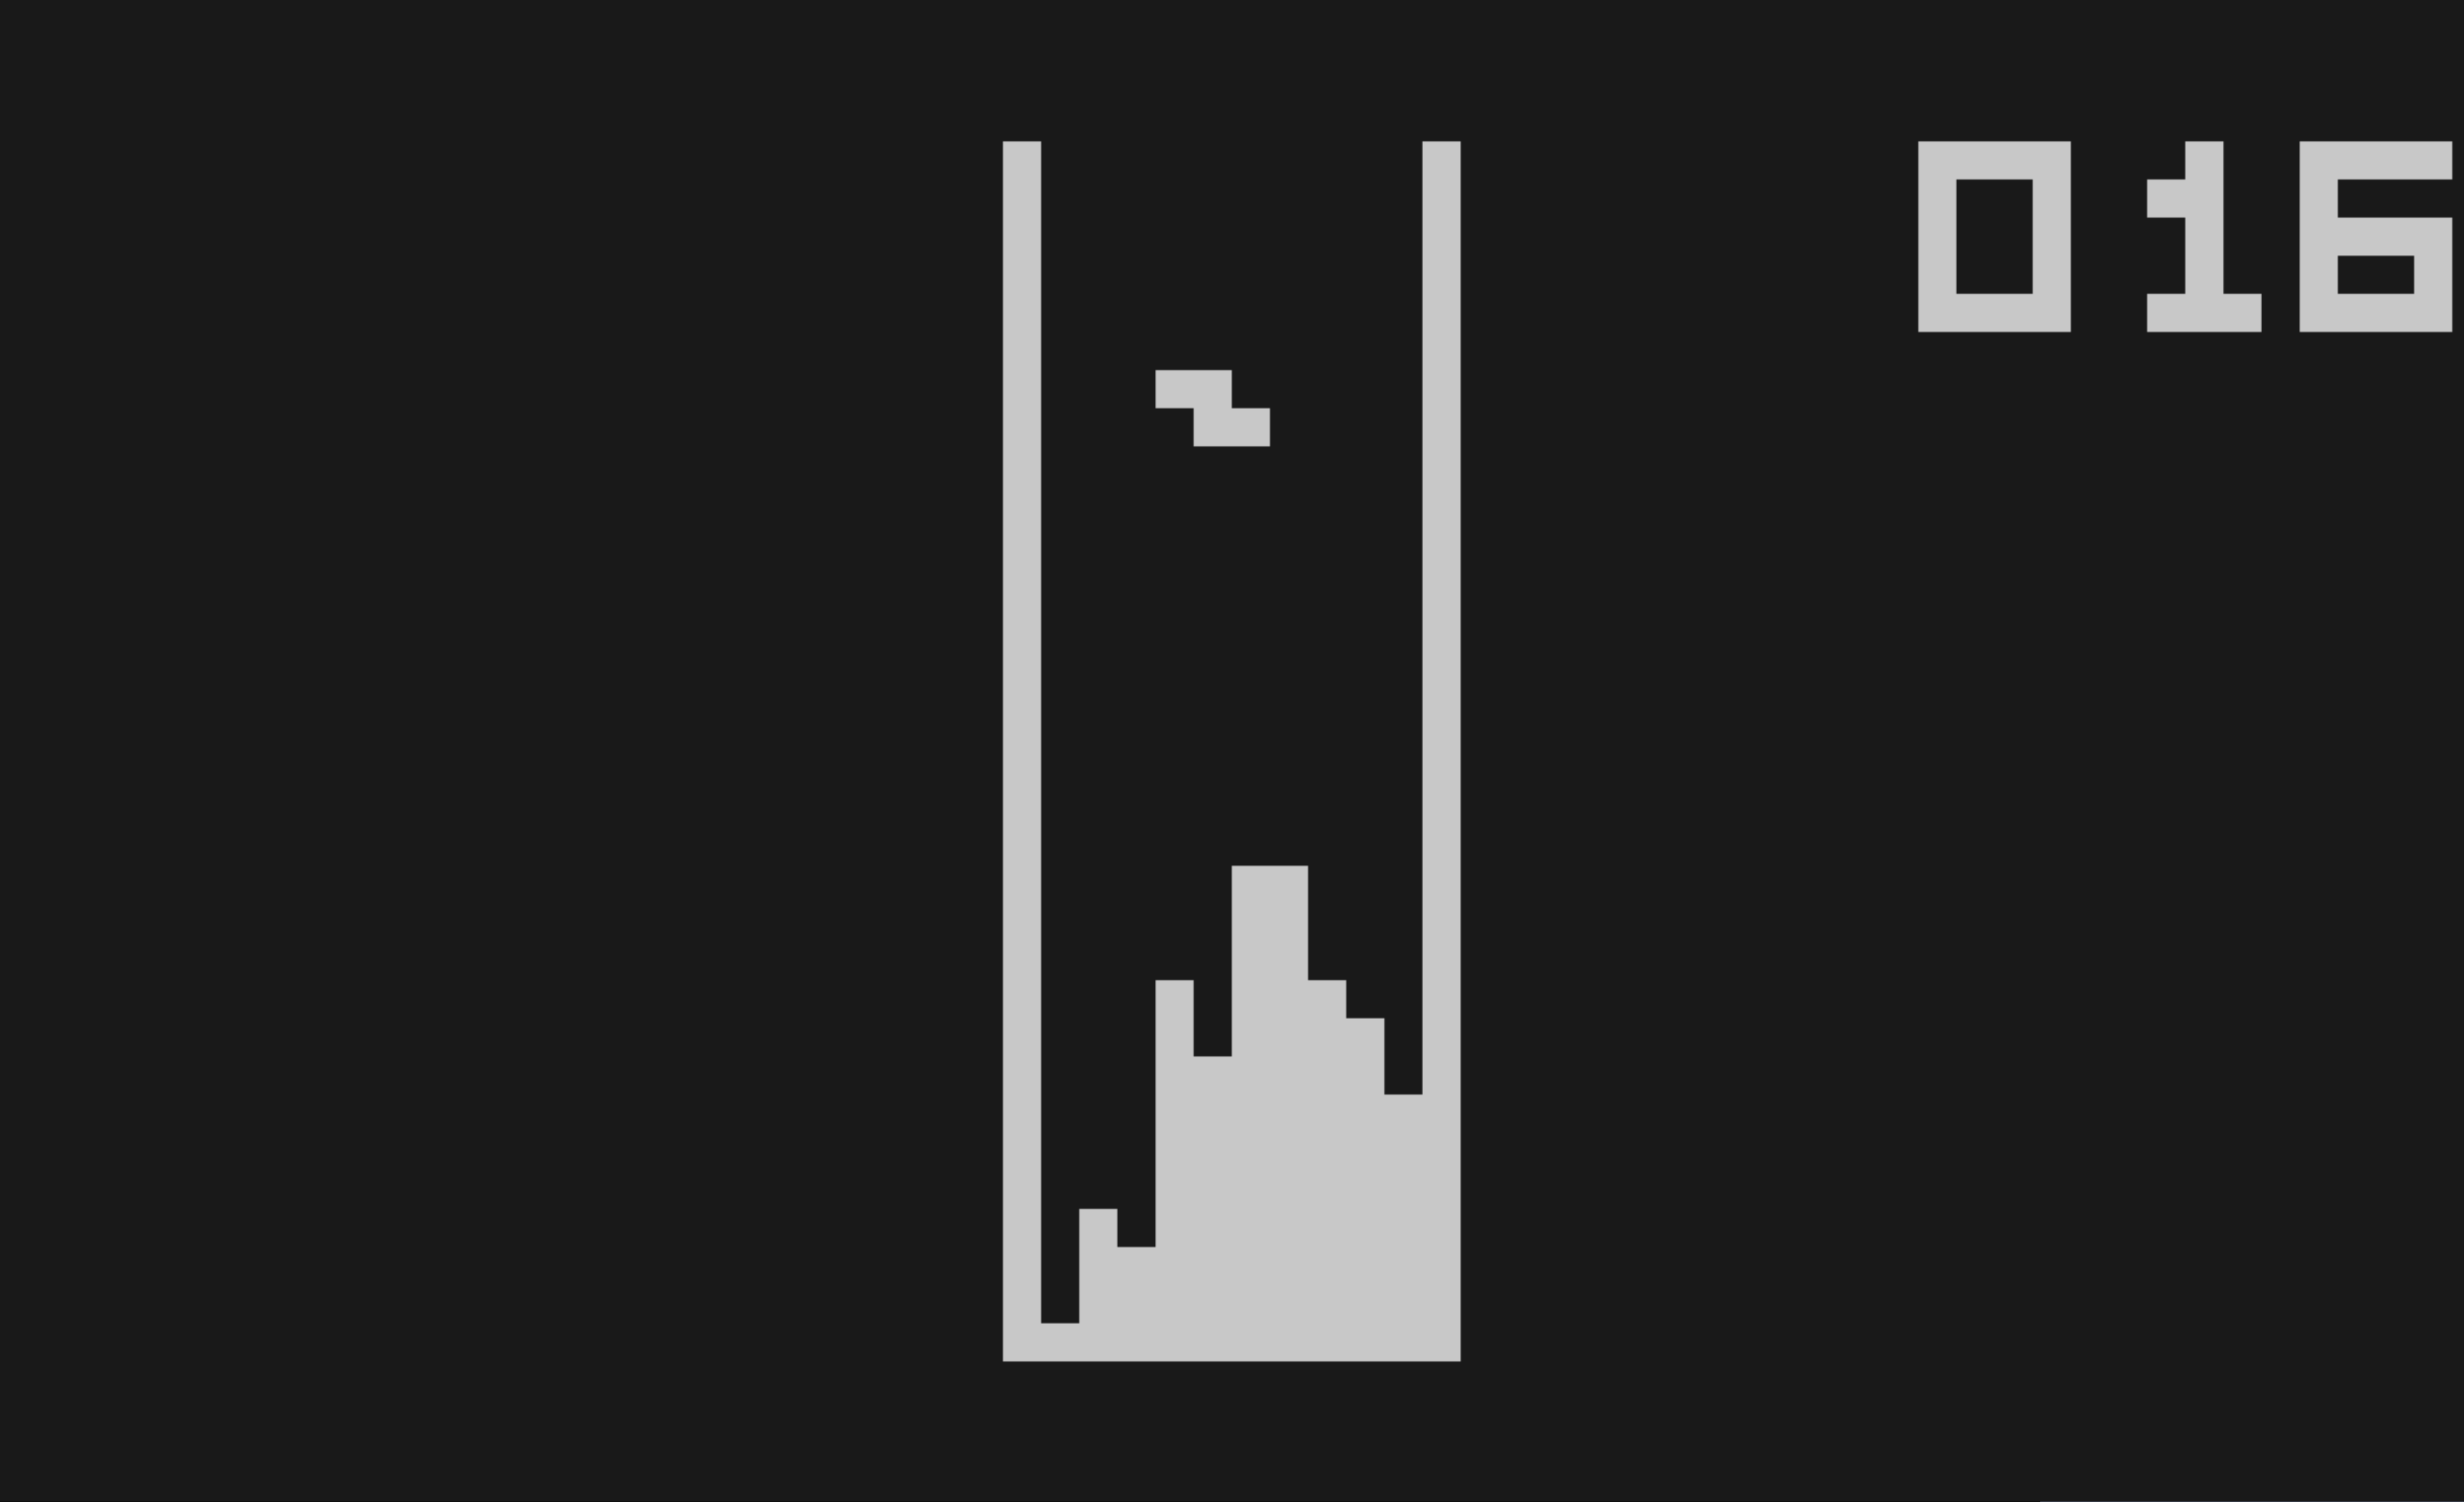
\includegraphics[width=\textwidth]{ch8/tetris}
\captionof{figure}{Tetris clone written in CHIP-8 by Fran Dachille in 1991 running in \texttt{Edra\ref{chap:ch4}}.}
\end{minipage}

\clearpage

\section{Virtual machine description}
\label{sec:ch3sec2}

\subsubsection{Memory}

\par The CHIP-8 virtual machine provides \textit{4KB} of accessible memory, reflecting the addressable range of its 16-bit memory registers. An exception to this is the \texttt{I} register, primarily utilized for drawing and memory operations, which is implemented as a 12-bit register rather than 16-bit. Multi-byte data within the system is stored in big-endian format, meaning the most significant byte precedes the least significant byte in memory.

\par Historically, the virtual machine's memory space overlapped with that of the interpreter, resulting in programs typically being loaded starting at address \texttt{0x200}. In contemporary implementations, this memory region is often repurposed to store font data, as emulators maintain separate memory spaces for code and data.

\par Furthermore, the uppermost \textit{256} bytes of memory (addresses \texttt{0xF00}-\texttt{0xFFF}) were originally allocated for display data. The adjacent lower segment (addresses \texttt{0xEA0}-\texttt{0xEFF}) was reserved for the interpreter's internal use, including the call stack and various system variables, though this reservation is frequently disregarded in modern emulator designs where the display data and emulator implementation is stored in a separate memory location.

\subsubsection{Registers}

\par The CHIP-8 virtual machine contains \textit{16} general-purpose 8-bit registers, labeled \texttt{V0} through \texttt{VF}. The \texttt{VF} register is reserved for use as a flag by certain instructions and should generally be avoided for storing general data, as its value may be altered implicitly during execution.

\subsubsection{Display}

\par The CHIP-8 display operates at a resolution of \texttt{64x32} pixels, rendering graphics in monochrome. Sprites are rendered onto the screen using a bitwise XOR based drawing method, whereby the sprite pixels are bitwise XORed with the existing framebuffer content. This technique allows for simple sprite toggling and erasure.

\par Additionally, the interpreter sets the flag register \texttt{VF} to \textit{1} if any pixel collision occurs during this process, specifically when a pixel is turned off as a result of overlapping pixels, providing a mechanism for collision detection in games and applications.

\begin{table}[H]
\centering
\begin{tabular}{
>{\columncolor[HTML]{333333}}l 
>{\columncolor[HTML]{333333}}l 
>{\columncolor[HTML]{333333}}l lllll
>{\columncolor[HTML]{EFEFEF}}l 
>{\columncolor[HTML]{EFEFEF}}l 
>{\columncolor[HTML]{EFEFEF}}l l
>{\columncolor[HTML]{333333}}l l
>{\columncolor[HTML]{333333}}l }
    &                          &  &  &  &                          &  &  &  &  &  &  &  & \cellcolor[HTML]{333333} &  \\
    & \cellcolor[HTML]{EFEFEF} &  &  &  & \cellcolor[HTML]{333333} &  &  &  &  &  &  &  &                          &  \\
\cellcolor[HTML]{EFEFEF} &
    &
    \cellcolor[HTML]{EFEFEF} &
    &
    \cellcolor[HTML]{333333} &
    \cellcolor[HTML]{333333} &
    \cellcolor[HTML]{333333} &
    &
    \cellcolor[HTML]{333333} &
    \cellcolor[HTML]{333333} &
    \cellcolor[HTML]{333333} &
    &
    &
    &
    \\
    & \cellcolor[HTML]{EFEFEF} &  &  &  & \cellcolor[HTML]{333333} &  &  &  &  &  &  &  &                          &  \\
    &                          &  &  &  &                          &  &  &  &  &  &  &  & \cellcolor[HTML]{333333} & 
\end{tabular}
\caption{Illustration of sprite XOR-ing, transforming an 8 (left) into a 0 (right), \texttt{VF} is set in this case to \textit{1}. The \textit{+} sign is not part of the sprite.}
\end{table}

\par The CHIP-8 virtual machine includes two timers: the delay timer and the sound timer. Both decrement at a fixed rate of \textit{60hz}. While the delay timer is typically used for timing-related logic within programs, the sound timer serves as an audio trigger. When the sound timer holds a non-zero value, it indicates that a sound should be produced.

\par The exact characteristics of the sound are not formally specified in the original CHIP-8 documentation, leaving its implementation to the discretion of the emulator developer. The most commonly adopted convention is to emulate the sound as a simple buzzer tone, consistent with the limitations of the original hardware.

\subsubsection{Input}

\par Input on the CHIP-8 system is handled via a hexadecimal keypad consisting of \textit{16} keys, labeled with values ranging from \textit{0} to \textit{F}.

\par A common convention is to arrange the keys in a 4 by 4 grid that mirrors the original layout, allowing intuitive input translation between physical keyboards and the virtual machine environment:

\begin{table}[H]
\centering
\begin{tabular}{| c | c | c | c |}
\hline
1 & 2 & 3 & C \\ \hline
4 & 5 & 6 & D \\ \hline
7 & 8 & 9 & E \\ \hline
A & 0 & B & F \\ \hline
\end{tabular}
\caption{Original input layout on the COSMAC VIP}
\end{table}

\begin{table}[H]
\centering
\begin{tabular}{| c | c | c | c |}
\hline
1 & 2 & 3 & 4 \\ \hline
Q & W & E & R \\ \hline
A & S & D & F \\ \hline
Z & X & C & V \\ \hline
\end{tabular}
\caption{Commonly used layout on modern keyboards}
\label{chip8:keyboard}
\end{table}

\subsubsection{Instructions \cite{CHIP8Gulrak}}

\begin{longtable}{|c|c|p{9cm}|}
\hline
\textbf{Opcode} & \textbf{Mnemonic} & \textbf{Description} \\
\hline
\endfirsthead

\hline
\textbf{Opcode} & \textbf{Mnemonic} & \textbf{Description} \\
\hline
\endhead

\hline
\endfoot

\hline
\endlastfoot

00E0 & CLS & Clear the display. \\
00EE & RET & Return from a subroutine. \\
1NNN & JP addr & Jump to location NNN. \\
2NNN & CALL addr & Call subroutine at NNN. \\
3XNN & SE Vx, byte & Skip next instruction if Vx is equal to NN. \\
4XNN & SNE Vx, byte & Skip next instruction if Vx is not equal to NN. \\
5XY0 & SE Vx, Vy & Skip next instruction if Vx is equal to Vy. \\
6XNN & LD Vx, byte & Set Vx = NN. \\
7XNN & ADD Vx, byte & Set Vx = Vx + NN. \\
8XY0 & LD Vx, Vy & Set Vx = Vy. \\
8XY1 & OR Vx, Vy & Set Vx = Vx OR Vy. \\
8XY2 & AND Vx, Vy & Set Vx = Vx AND Vy. \\
8XY3 & XOR Vx, Vy & Set Vx = Vx XOR Vy. \\
8XY4 & ADD Vx, Vy & Set Vx = Vx + Vy, set VF = carry. \\
8XY5 & SUB Vx, Vy & Set Vx = Vx - Vy, set VF = NOT borrow. \\
8XY6 & SHR Vx {, Vy} & Set Vx = Vx SHR 1. \\
8XY7 & SUBN Vx, Vy & Set Vx = Vy - Vx, set VF = NOT borrow. \\
8XYE & SHL Vx {, Vy} & Set Vx = Vx SHL 1. \\
9XY0 & SNE Vx, Vy & Skip next instruction if Vx is not equal to Vy. \\
ANNN & LD I, addr & Set I = NNN. \\
BNNN & JP V0, addr & Jump to location NNN + V0. \\
CXNN & RND Vx, byte & Set Vx = random byte AND NN. \\
DXYN & DRW Vx, Vy, nibble & Display n-byte sprite starting at memory location I at (Vx, Vy), set VF = collision. \\
EX9E & SKP Vx & Skip next instruction if key with the value of Vx is pressed. \\
EXA1 & SKNP Vx & Skip next instruction if key with the value of Vx is not pressed. \\
FX07 & LD Vx, DT & Set Vx = delay timer value. \\
FX0A & LD Vx, K & Wait for a key press, store the value of the key in Vx. \\
FX15 & LD DT, Vx & Set delay timer = Vx. \\
FX18 & LD ST, Vx & Set sound timer = Vx. \\
FX1E & ADD I, Vx & Set I = I + Vx. \\
FX29 & LD F, Vx & Set I = location of sprite for digit Vx. \\
FX33 & LD B, Vx & Store BCD representation of Vx in memory locations I, I+1, and I+2. \\
FX55 & LD [I], Vx & Store registers V0 through Vx in memory starting at location I. \\
FX65 & LD Vx, [I] & Read registers V0 through Vx from memory starting at location I. \\
\end{longtable}

\par The original CHIP-8 implementation supported a total of 35 instructions, although only 31 were explicitly documented in the initial specification. Notably, opcodes such as \texttt{8XY3}, \texttt{8XY6}, \texttt{8XY7}, and \texttt{8XYE} were omitted from the formal documentation.

\par This omission is likely attributable to the historical context of CHIP-8’s design, which was implemented atop the RCA 1802 microprocessor. The \texttt{8XY*} instruction group closely mirrors operations available in the 1802’s Arithmetic Logic Unit (ALU), suggesting that these opcodes may have originated from the hardware's native capabilities rather than being explicitly defined by the CHIP-8 interpreter itself.

\par Subsequent extensions to the CHIP-8 instruction set, such as those introduced in SCHIP (Super CHIP) and other variants, have redefined or augmented the behavior of certain instructions. For example, instructions \texttt{FX55} and \texttt{FX65} originally incremented the index register \texttt{I} after each memory write or read, respectively. However, later implementations, including SCHIP, omit this side effect, reflecting divergence in interpretation and a lack of standardization across extensions, which will be discussed later.

\section{Emulator implementation}
\label{sec:ch3sec3}

\par The core CHIP-8 library, \texttt{cchip8\cite{GithubCCHIP8}}, is organized into modular components: the state, the interpreter, and the static compiler. This architecture enforces a clear separation of concerns, where only the execution runners depend on the state module, and each module operates independently, promoting maintainability and extensibility.

\par The state module, defined in the file \texttt{state.h}, functions as the central interface between the emulator core and the external environment. It encapsulates the full virtual machine state as well as a set of callback function pointers that enable host-controlled behavior, such as memory access, rendering, input handling, and random number generation.

\par The \texttt{chip8\_state}'s structure maintains essential CHIP-8 runtime components, including program counter (\texttt{pc}), index register (\texttt{i}), stack and stack pointer (\texttt{stack}, \texttt{sp}), \textit{16} general-purpose registers (\texttt{v[0x10]}), timers (\texttt{dt}, \texttt{st}), display resolution parameters, and font memory addresses.

\par In addition, it includes a flag \texttt{draw\_flag} for screen redraw signaling and a variable \texttt{last\_key} to track the most recently pressed key to emulate accurate behaviour for the \textit{FX0A} instruction family.

\par The embedded function pointers (\texttt{read\_b}, \texttt{read\_w}, \texttt{write\_b}, etc.) abstract interactions with the host system. These allow the emulator to delegate low-level operations such as I/O, drawing, screen clearing, input polling, and random number generation to external implementations, facilitating portability and customization.

\par An auxiliary argument pointer (\texttt{aux\_arg}) is also provided to pass user-defined data to these callbacks, supporting more complex execution contexts if needed.

\begin{minted}[
    linenos,                % add line numbers
    fontfamily=tt,          % typewriter font
    fontsize=\small,        % size
    breaklines,             % allow line breaks
    tabsize=4               % size of tab
]{C}
struct chip8_state
{
    bool draw_flag;
    chip8_run_mode_t mode;
    uint16_t pc, i, stack[0x100];
    uint8_t display_width, display_height;
    uint8_t v[0x10], sp, dt, st, last_key;
    uint16_t lowres_font_address, hires_font_address;
    
    // Callbacks.
    chip8_read_b_f read_b;
    chip8_read_w_f read_w;
    chip8_write_b_f write_b;
    chip8_draw_sprite_f draw_sprite;
    chip8_clear_f clear_screen;
    chip8_key_status_f get_key_status;
    chip8_random_f get_random;
    chip8_resize_f resize;
    chip8_scroll_f scroll;
    
    void* aux_arg;  // Used for passing data to the callbacks.
};
\end{minted}

\subsection{Interpreter}
\label{subsec:ch3sec3sub1}

\par The interpreter, as defined in the file \texttt{cpu/interpreter.h}, encapsulates a minimal runtime structure responsible for controlling instruction execution.

\par The \texttt{chip8\_interpreter\_t} struct maintains three key fields: a boolean flag \texttt{running} to indicate whether the interpreter is actively executing instructions, a \texttt{long} field \texttt{timer} to track internal timing mechanisms, and a pointer \texttt{state} to the shared \texttt{chip8\_state\_t} structure, which contains the core emulator state, mentioned above.

\begin{minted}[
    linenos,                % add line numbers
    fontfamily=tt,          % typewriter font
    fontsize=\small,        % size
    breaklines,             % allow line breaks
    tabsize=4               % size of tab
]{C}
typedef struct chip8_interpreter
{
    bool running;
    long timer;
    chip8_state_t* state;
} chip8_interpreter_t;
\end{minted}

\par This design ensures that the interpreter remains lightweight, delegating system-wide responsibilities to the state module while managing control flow and timing locally, and such, enables the interpreter to operate independently of the underlying platform or user interface, facilitating reuse and testing.

\par The main function \texttt{chip8\_interpreter\_step(chip8\_interpreter\_t* self)} is responsible for executing a single instruction cycle within the interpreter. It represents the core of the CHIP-8 execution loop, fetching the current instruction from memory, decoding it, and dispatching it for execution.

\par Internally, instruction decoding is implemented using a large \texttt{switch} statement, a common pattern in interpreter design, especially for simpler architectures. The instruction opcode, 16 bits in CHIP-8, is fetched from memory using the program counter (\texttt{pc}) and then used to determine which operation to execute.

\par Each \texttt{case} in the \texttt{switch} corresponds to a specific opcode or opcode pattern, allowing for structured, readable, and performant instruction handling.

\par This dispatch method, while straightforward, also benefits from modern compiler optimizations that often convert large \texttt{switch} statements into jump tables, providing relatively fast execution times.

\par Additionally, this layout makes it easier to maintain and extend the interpreter, as new opcodes can be added with minimal structural disruption.

\section{Quirks and extensions}
\label{sec:ch3sec4}

\subsection{Modern Super CHIP-8}
\label{subsec:ch3sec4sub1}

\begin{minipage}{\linewidth}

\includegraphics[width=\textwidth]{ch8/octogon}
\centering
\captionof{figure}{Octogon by John Earnest running in \texttt{Edra\ref{chap:ch4}}'s modern SCHIP mode.\\}
\end{minipage}

\par The Super-CHIP (SCHIP) extension, introduced by Erik Bryntse in the 1990s, builds upon the original CHIP-8 virtual machine to enhance its graphical capabilities and improve overall program flexibility.

\par The most notable addition is the expansion of the display resolution from \texttt{64x32} pixels to \texttt{128x64} pixels, enabling more detailed graphics.

\par SCHIP also introduces a set of extended instructions\cite{CHIP8Gulrak}, particularly for drawing and scrolling operations, as well as instructions to modify the behavior of the display or interpreter, the ones implemented in \texttt{Edra\ref{chap:ch4}} are as follows:

\begin{longtable}{|c|p{10cm}|}
\hline
\textbf{Opcode} & \textbf{Description} \\
\hline
\endfirsthead

\hline
\textbf{Opcode} & \textbf{Description} \\
\hline
\endhead

\hline
\endfoot

\hline
\endlastfoot

00CN & Scroll display down by \texttt{n} pixels. \\
00FB & Scroll display right by 4 pixels. \\
00FC & Scroll display left by 4 pixels. \\
00FD & Exit the interpreter (halt). \\
00FE & Enable low-resolution mode (64x32). \\
00FF & Enable high-resolution mode (128x64). \\
DXY0 & Draw 16x16 sprite in high-resolution mode. In low-res mode, behaves like standard DXYN. \\
\end{longtable}

\section{Testing}
\label{sec:ch3sec5}

\par The current implementation has been tested for correctness using \texttt{Timendus' CHIP8 test suite\cite{CHIP8Timendus}}, a well known test suite in the community. It assures correct behaviour, identical to the original implementation unless otherwise specified. 

\par The suite supports tests from the smallest subset of the instructions that could be implemented, enough for an image of the IBM logo to be displayed:

\begin{longtable}{|c|l|}
\hline
\textbf{Opcode} & \textbf{Description} \\ \hline
\endfirsthead

\hline
\textbf{Opcode} & \textbf{Description} \\ \hline
\endhead

\hline
\endfoot

\hline
\endlastfoot

00E0 & Clear the screen.                                        \\ \hline
6XNN & Load normal register with immediate value.               \\ \hline
ANNN & Load index register with immediate value.                \\ \hline
7XNN & Add immediate value to normal register.                  \\ \hline
DXYN & Draw sprite to screen (unaligned, easier to implement).  \\ \hline
1NNN & Jump (optional, only at the end).                        \\
\end{longtable}

\begin{minipage}{\linewidth}

\includegraphics[width=\textwidth]{ch8/ibm}
\centering
\captionof{figure}{The IBM logo display running in \texttt{Edra\ref{chap:ch4}} showing the correct result.\\}
\end{minipage}

\clearpage

\par To the entire instruction set and the correct hardware timings and quirks, including the flags set by the instructions:\\

\begin{minipage}{\linewidth}
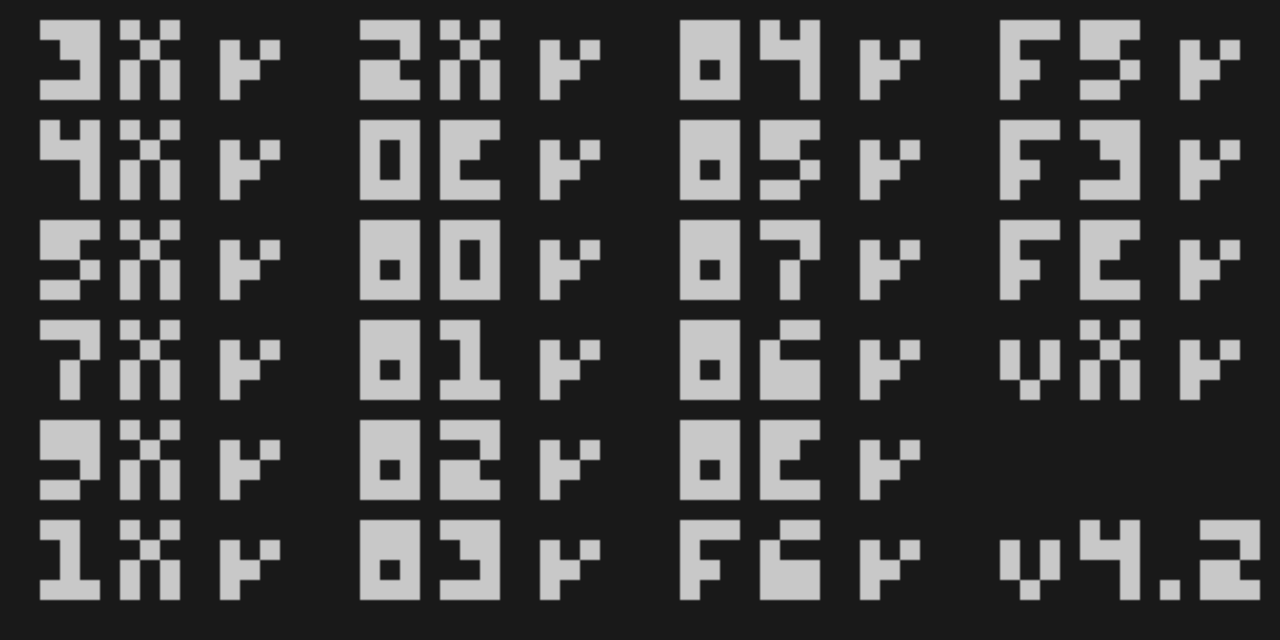
\includegraphics[width=\textwidth]{ch8/corax}
\end{minipage}

\begin{minipage}{\linewidth}
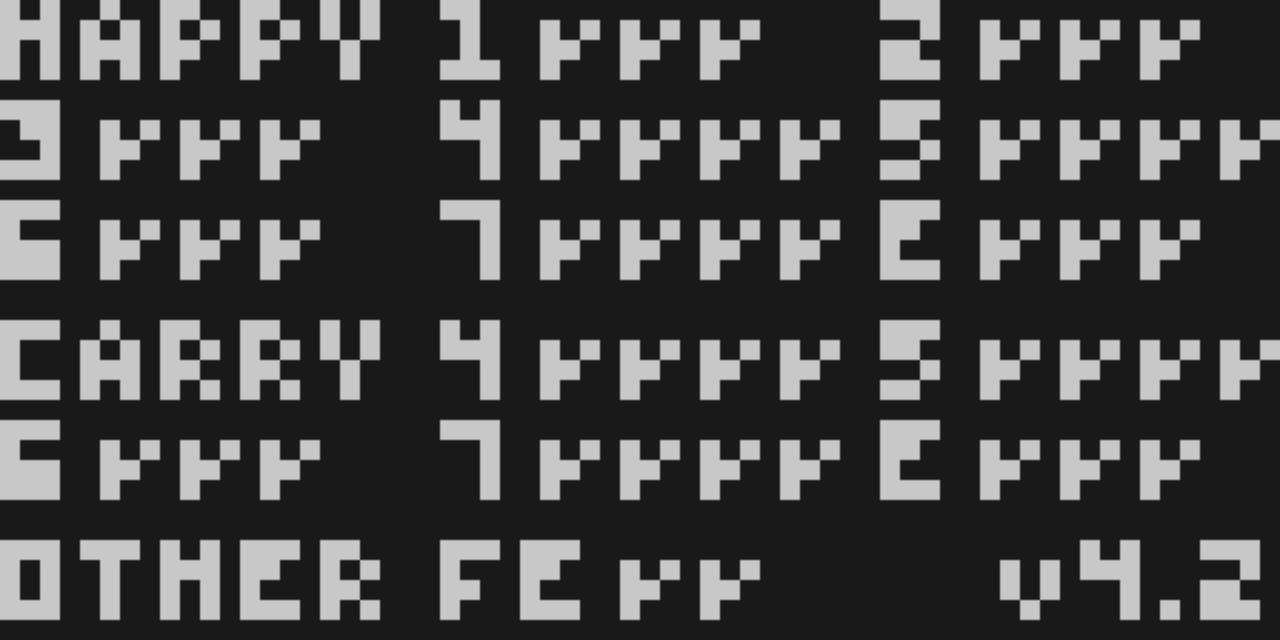
\includegraphics[width=\textwidth]{ch8/flags}
\centering
\captionof{figure}{The Corax+ opcode and the flags tests running in \texttt{Edra\ref{chap:ch4}} showing the correct result.\\}
\end{minipage}

\clearpage

\par These tests have been ran manually in all possible configurations to make sure the emulator is behaving as expected, even in modern SCHIP mode.\\

\begin{minipage}{\linewidth}
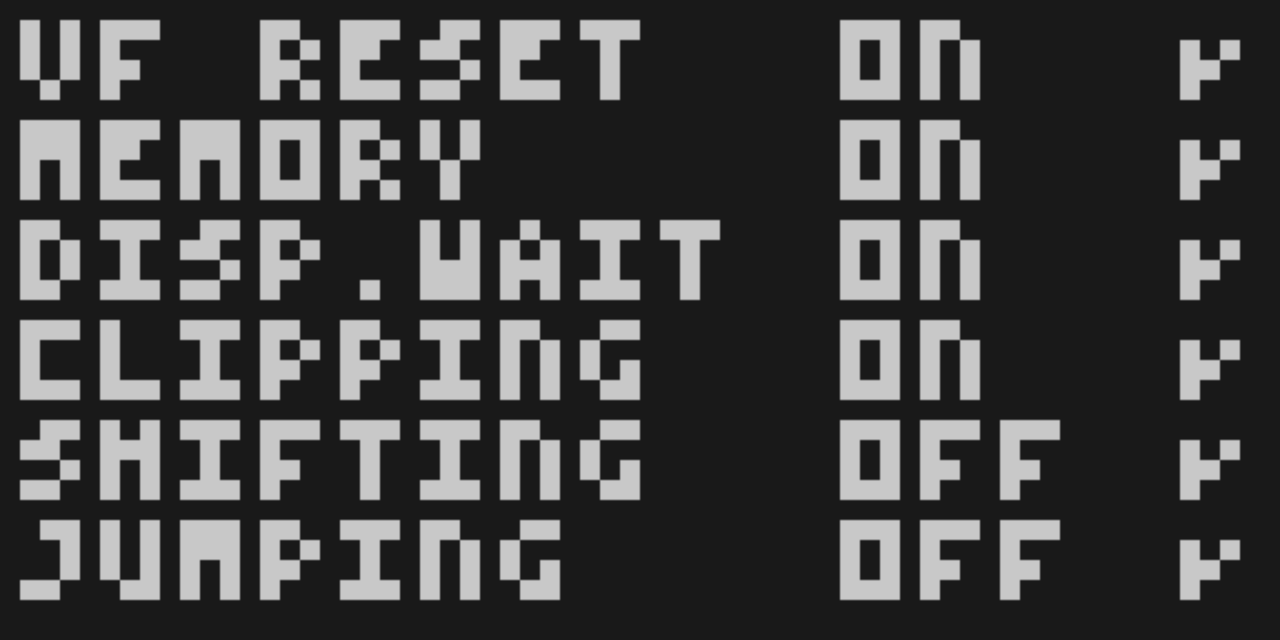
\includegraphics[width=\textwidth]{ch8/quirks-normal}
\end{minipage}

\begin{minipage}{\linewidth}
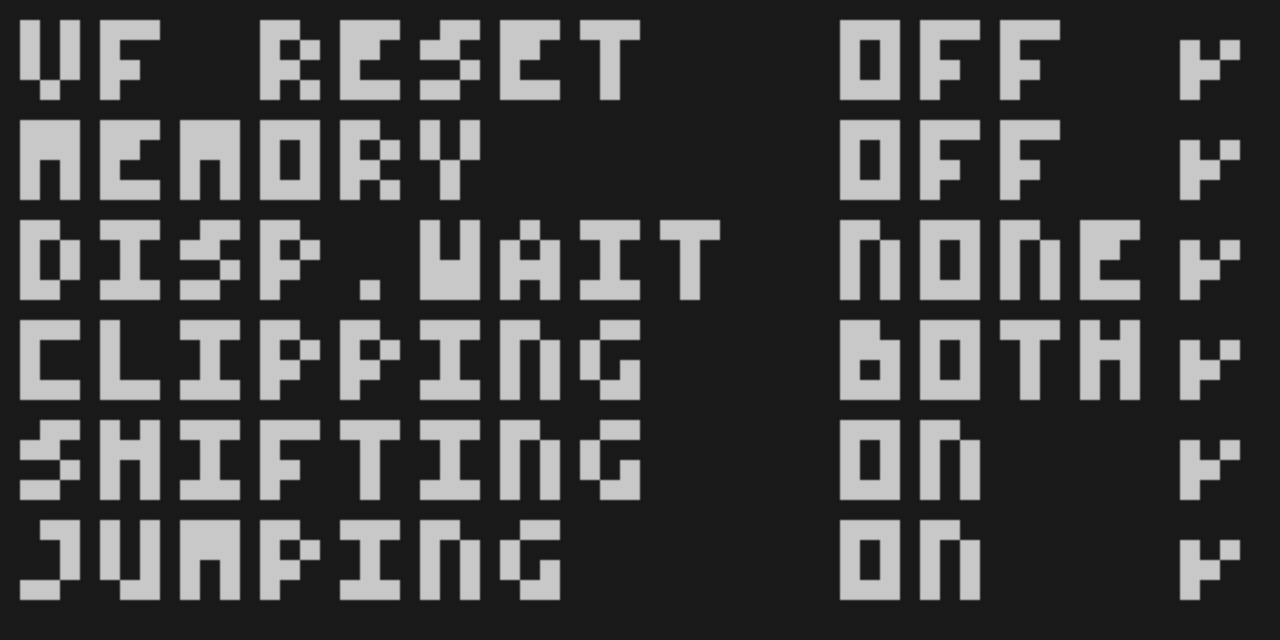
\includegraphics[width=\textwidth]{ch8/quirks-schip}
\centering
\captionof{figure}{The quirks test, normal CHIP8 and modern SCHIP variants running in \texttt{Edra\ref{chap:ch4}} showing the correct result for each of the respective platforms. \\}
\end{minipage}
\chapter{The final application}
\label{chap:ch4}

\par The application, called \href{https://github.com/solomonarul/edra}{\texttt{Edra}}, has been designed from the outset with a primary focus on performance, emphasizing both speed and low latency. To meet these requirements, the C programming language was selected for the development of the emulator, due to its low-level access to system resources and minimal runtime overhead.

\par For graphical output and user interaction, the \href{https://wiki.libsdl.org/SDL3/FrontPage}{\texttt{SDL3}} library was chosen for its cross-platform compatibility, lightweight nature, and ease of integration into C-based projects.

\par When evaluating options for graphical user interface (GUI) development in pure C, the available choices were rather limited. The GUI development space is predominantly occupied by C++ libraries such as \href{https://github.com/ocornut/imgui}{\textit{ImGui}}, which are not directly compatible with C without the use of external bindings which would make the development process rather complicated.

\par Ultimately, the project adopted the \href{https://github.com/nicbarker/clay}{\texttt{clay}} library, a platform-agnostic C layout engine. This library facilitates GUI construction by generating a series of rendering operations that can be implemented using a backend such as \href{https://wiki.libsdl.org/SDL3/FrontPage}{\texttt{SDL3}}, thereby enabling flexible and portable UI rendering within the application.

\section{Design and implementation}
\label{sec:ch4sec1}

\par The emulator's core functionality was subsequently modularized into a dedicated git submodule, referred to as \href{https://github.com/solomonarul/cchip8}{\texttt{cchip8}}, located in the \textit{lib/cchip8} directory. This module encapsulates all fundamental components required for CHIP8 emulation.

\par Building upon this foundation, the CHIP8 driver, located in \textit{drivers/chip8}, instantiates a machine capable of loading and executing CHIP8 programs.

\par This virtual machine is then integrated into an application state, which is responsible for managing its output within the broader context of \href{https://github.com/solomonarul/edra}{\texttt{Edra}}'s state management system.

\par Similarly, the Brainfuck emulator has its own module called \href{https://github.com/solomonarul/cbf}{\texttt{cbf}} available at \textit{lib/cbf} which handles all of the components necessary for the machine at \textit{drivers/cbf} which is then used by the state in the app.

\par For cross-platform non-standard features, such as dynamic arrays, .ini file parsing and so on, custom implementations have been made and separated into their own separate module called \href{https://github.com/solomonarul/auxum}{\texttt{auxum}} available in the \textit{lib/auxum} folder.

\begin{figure}[htbp]
\centering
\begin{tikzpicture}[
    state/.style={rectangle, draw, thick, minimum width=3cm, minimum height=1cm, align=center},
    arrow/.style={-Stealth, thick}
]

% Initial state
\node[state] (initial) {\texttt{chip8\_state\_t}};
\node[below=0.2cm of initial] (label1) {Initial State};

% Pressing Enter
\node[above=1.2cm of initial] (action1) {Pressing Escape};
\draw[arrow] (initial.north) -- (action1.south);

% Paused state
\node[state, above=1cm of action1] (paused) {\texttt{chip8\_pause\_state\_t}};
\node[state, below=0.1cm of paused] (initial2) {\texttt{chip8\_state\_t}};
\node[right=0.2cm of initial2] (label2) {Paused State};

% Pressing Esc
\node[above=1.2cm of paused] (action2) {Pressing Escape};
\draw[arrow] (paused.north) -- (action2.south);

% Return to initial
\node[state, above=1cm of action2] (final) {\texttt{chip8\_state\_t}};
\node[below=0.2cm of final] (label3) {Initial State Restored};

% Return arrow
\draw[arrow, dashed] (final.east) to[out=0, in=0, looseness=1.5] (initial.east);

\end{tikzpicture}
\caption{Stack-based state transitions, as used in the app.}\label{fig:state_stack}
\end{figure}

\section{Porting and compiling}
\label{sec:ch4sec2}

\par During cross-platform porting efforts, several implementation constraints necessitated platform-specific adaptations:
\begin{itemize}
    \item \textit{PlayStation Vita}: JIT emulation was disabled due to the absence of POSIX-compliant threading support, which prevented successful compilation of the GNU Lightning library. Additionally, memory allocation thresholds required modification within the VitaSDK framework, as implemented in \href{https://github.com/solomonarul/auxum/blob/main/inc/auxum/platform/vita/heap.h}{\texttt{auxum}.}
    \item \textit{Microsoft Windows}: JIT functionality was similarly disabled following segmentation faults during compilation attributed to GNU Lightning incompatibilities, potentially stemming from toolchain limitations within the GCC Windows environment.
    \item \textit{Linux}: Full functionality was maintained without modification, demonstrating native compatibility with the implementation's architectural dependencies.
\end{itemize}

\par To facilitate compilation, a standardized build system was implemented using \texttt{Make}. This system provides template commands for all supported platforms, as documented in the project's \href{https://github.com/solomonarul/edra}{\texttt{GitHub repository}}:

\begin{enumerate}
    \item \textit{Environment Configuration}: Specify \texttt{SDL3\_DIR} and \texttt{SDL3\_TTF\_DIR} variables in CMake's build cache when required for dependency resolution.
    
    \item \textit{Platform-Specific Compilation}: Execute the appropriate build command:\\\textit{  make b\{platform\}\{configuration\}}
    \begin{itemize}
        \item \texttt{platform} denotes the target system:
        \begin{itemize}
            \item \texttt{w}: Microsoft Windows
            \item \texttt{u}: Unix-like systems (Linux, BSD)
            \item \texttt{v}: PlayStation Vita
        \end{itemize}
        \item \texttt{configuration} specifies the build type:
        \begin{itemize}
            \item \texttt{d}: Debug build
            \item \texttt{r}: Release build
        \end{itemize}
    \end{itemize}
\end{enumerate}

\clearpage

\section{Usage}
\label{sec:ch4sec3}

\subsubsection{GUI}
\label{sec:ch4sec4subsub1}

\begin{minipage}{\linewidth}
\centering
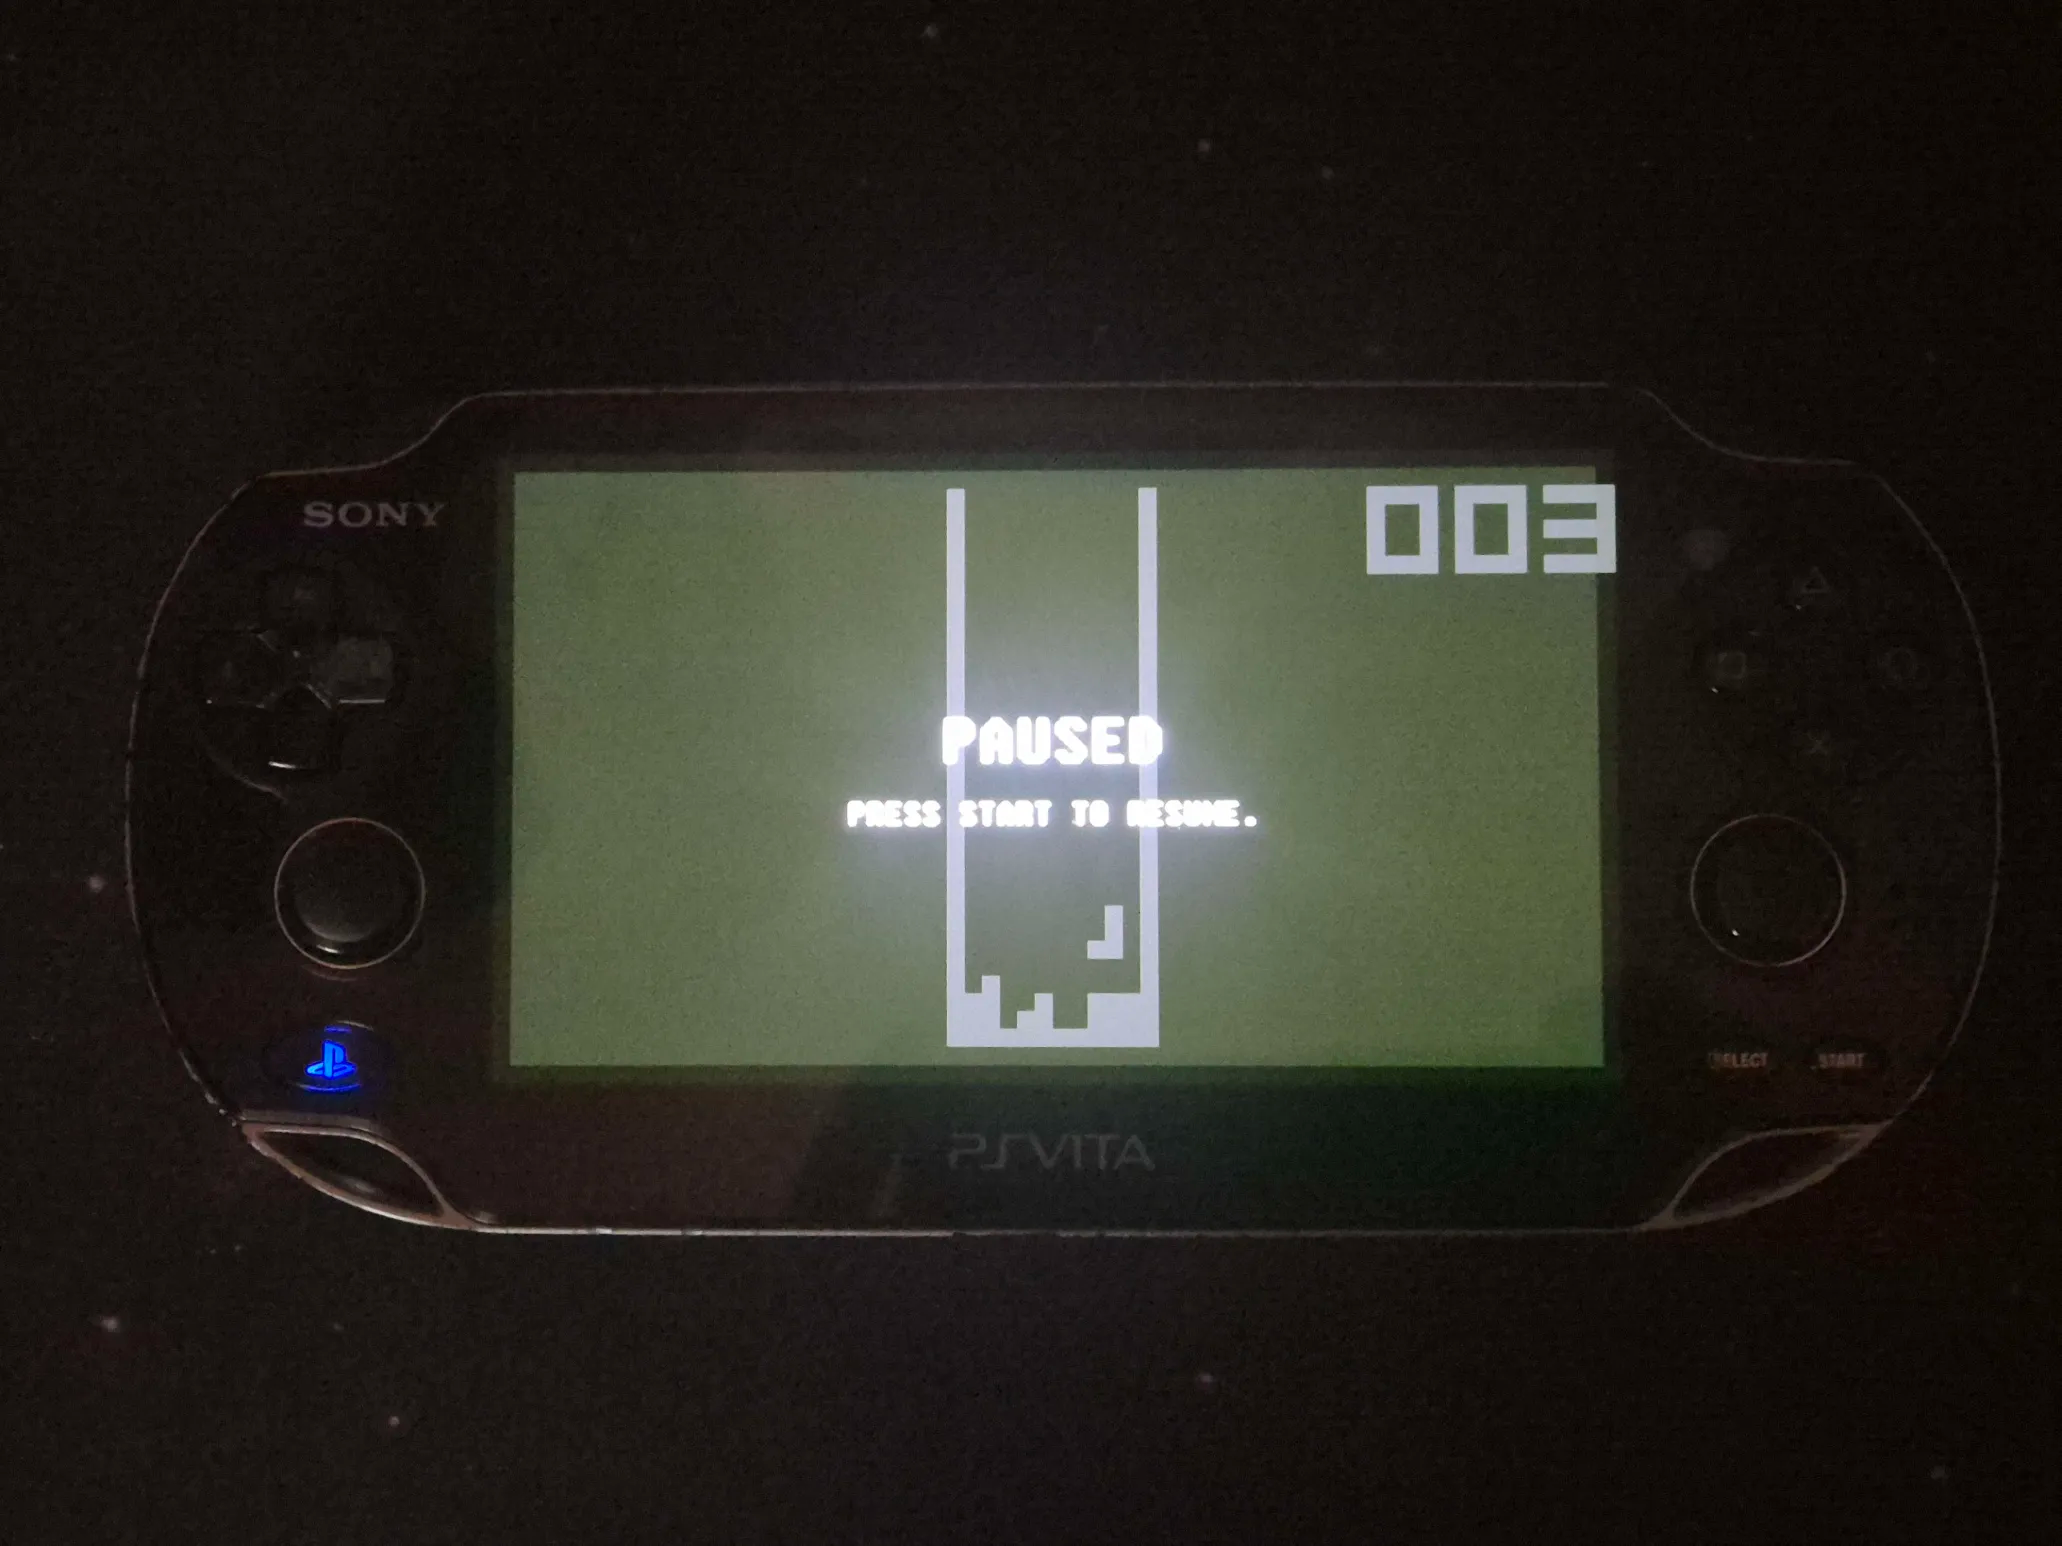
\includegraphics[width=0.75\textwidth]{app/vita}
\captionof{figure}{The app running on a PlayStation Vita system.}
\end{minipage}

\begin{minipage}{\linewidth}
\centering

\includegraphics[width=0.66\textwidth]{app/normal}
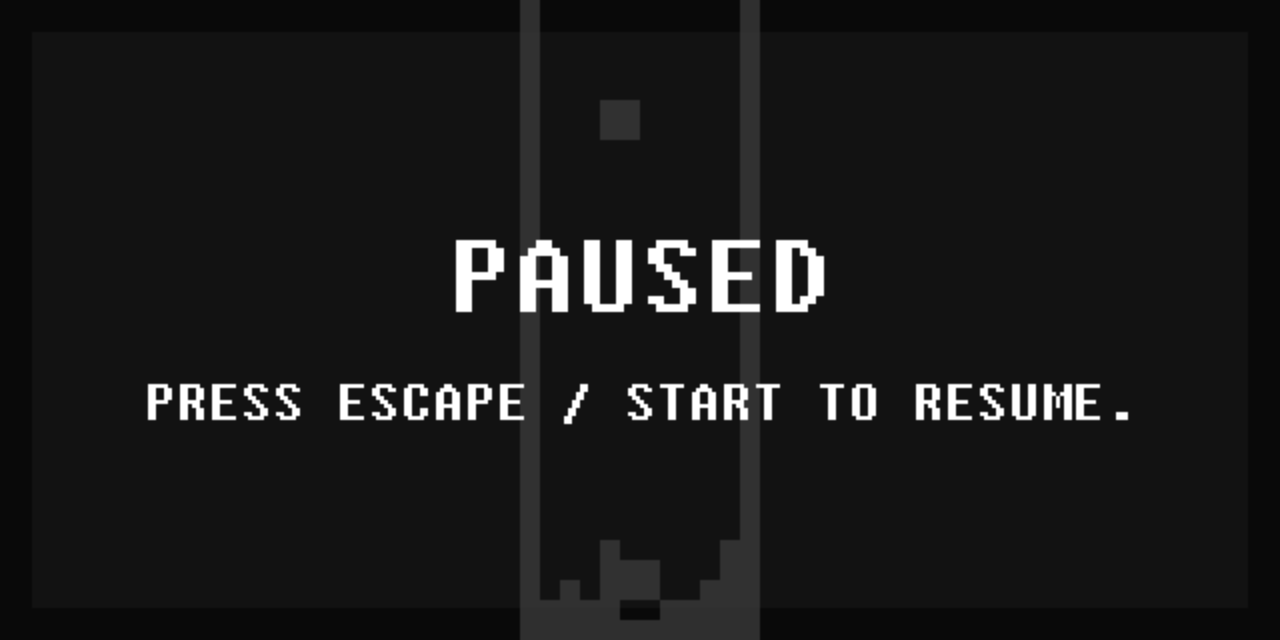
\includegraphics[width=0.66\textwidth]{app/pause}
\captionof{figure}{The app being paused by pressing Escape or Start on a gamepad.}
\end{minipage}
\clearpage

\chapter{Conclusions and Future Work}
\label{conclusions}

\par This thesis has systematically explored the design, implementation, and performance trade-offs between interpretation and just-in-time (JIT) compilation for software emulation, using the minimalist languages \textit{Brainfuck} and \textit{CHIP-8} as pedagogical case studies.

\par The key findings demonstrate that \textit{JIT compilation consistently outperforms interpretation}, particularly for computationally intensive or long-running programs, due to the elimination of repetitive instruction fetching and decoding overhead. Empirical benchmarks revealed execution times as low as \textit{3--9\% of interpreter runtimes} for Brainfuck programs.

\par Optimizations such as \textit{instruction folding}, \textit{precalculated jumps}, and \textit{hot loop replacement} proved highly effective, though diminishing returns were observed with excessive specialization. For instance, overly aggressive loop collapsing occasionally generated machine code identical to unoptimized sequences, increasing complexity without performance gains. This underscores the importance of \textit{balancing optimization effort with practical returns}, especially in constrained environments.

\par The modular architecture of the final application, \textit{Edra}, successfully decoupled emulation logic (via \texttt{cbf} and \texttt{cchip8} libraries) from platform-specific I/O (using SDL3 and Clay), enabling portable CHIP-8 and Brainfuck emulation. Test validation with established suites (e.g., Timendus\cite{CHIP8Timendus} for CHIP-8) confirmed correctness across standard and extended specifications like SCHIP.

\subsection*{Future Work}

\par Several avenues merit further exploration:

\begin{enumerate}
    \item \textit{Better User Experience}: Improved GUI with program selection and configurable in-app settings.
    \item \textit{Broader Language Support}: Extending the framework to emulate more complex architectures (e.g. 6502, Z80, etc).
    \item \textit{More platforms supported}: Emulating game consoles / platforms that have already had their architecture reverse engineered and are openly available (e.g. Nintendo GameBoy, etc)
\end{enumerate}

\bibliography{../references}

\end{document}
